\begin{figure}
	\centering
	\begin{tikzpicture}[scale = 5]
	\tikzstyle{VertexStyle} = []
	\tikzstyle{EdgeStyle} = []
	\tikzstyle{labeledStyle}=[shape = circle, minimum size = 6pt, inner sep = 1.2pt, draw]
	\tikzstyle{unlabeledStyle}=[shape = circle, minimum size = 6pt, inner sep = 1.2pt, draw, fill]
	\Vertex[style = labeledStyle, x = 0.300, y = 0.250, L = \small {$0$}]{v0}
	\Vertex[style = labeledStyle, x = 0.700, y = 0.250, L = \small {$0$}]{v1}
	\Vertex[style = labeledStyle, x = 0.500, y = 0.500, L = \small {$1$}]{v2}
	\Vertex[style = labeledStyle, x = 0.500, y = 0.250, L = \small {$0$}]{v3}
	\Edge[label = \small {}, labelstyle={auto=right, fill=none}](v0)(v2)
	\Edge[label = \small {}, labelstyle={auto=right, fill=none}](v0)(v3)
	\Edge[label = \small {}, labelstyle={auto=right, fill=none}](v1)(v2)
	\Edge[label = \small {}, labelstyle={auto=right, fill=none}](v1)(v3)
	\Edge[label = \small {}, labelstyle={auto=right, fill=none}](v2)(v3)
	\end{tikzpicture}\hspace{.3in}
\begin{tikzpicture}[scale = 5]
\tikzstyle{VertexStyle} = []
\tikzstyle{EdgeStyle} = []
\tikzstyle{labeledStyle}=[shape = circle, minimum size = 6pt, inner sep = 1.2pt, draw]
\tikzstyle{unlabeledStyle}=[shape = circle, minimum size = 6pt, inner sep = 1.2pt, draw, fill]
\Vertex[style = labeledStyle, x = 0.750, y = 0.500, L = \small {$1$}]{v0}
\Vertex[style = labeledStyle, x = 0.900, y = 0.250, L = \small {$0$}]{v1}
\Vertex[style = labeledStyle, x = 0.600, y = 0.250, L = \small {$0$}]{v2}
\Vertex[style = labeledStyle, x = 1.050, y = 0.250, L = \small {$0$}]{v3}
\Vertex[style = labeledStyle, x = 0.750, y = 0.250, L = \small {$0$}]{v4}
\Edge[label = \small {}, labelstyle={auto=right, fill=none}](v0)(v2)
\Edge[label = \small {}, labelstyle={auto=right, fill=none}](v0)(v3)
\Edge[label = \small {}, labelstyle={auto=right, fill=none}](v0)(v4)
\Edge[label = \small {}, labelstyle={auto=right, fill=none}](v1)(v3)
\Edge[label = \small {}, labelstyle={auto=right, fill=none}](v1)(v4)
\Edge[label = \small {}, labelstyle={auto=right, fill=none}](v2)(v4)
\end{tikzpicture}\hspace{.3in}
\begin{tikzpicture}[scale = 5]
\tikzstyle{VertexStyle} = []
\tikzstyle{EdgeStyle} = []
\tikzstyle{labeledStyle}=[shape = circle, minimum size = 6pt, inner sep = 1.2pt, draw]
\tikzstyle{unlabeledStyle}=[shape = circle, minimum size = 6pt, inner sep = 1.2pt, draw, fill]
\Vertex[style = labeledStyle, x = 0.450, y = 0.700, L = \small {$1$}]{v0}
\Vertex[style = labeledStyle, x = 0.300, y = 0.400, L = \small {$0$}]{v1}
\Vertex[style = labeledStyle, x = 0.600, y = 0.400, L = \small {$0$}]{v2}
\Vertex[style = labeledStyle, x = 0.150, y = 0.400, L = \small {$0$}]{v3}
\Vertex[style = labeledStyle, x = 0.750, y = 0.400, L = \small {$0$}]{v4}
\Vertex[style = labeledStyle, x = 0.450, y = 0.400, L = \small {$0$}]{v5}
\Edge[label = \small {}, labelstyle={auto=right, fill=none}](v0)(v3)
\Edge[label = \small {}, labelstyle={auto=right, fill=none}](v0)(v4)
\Edge[label = \small {}, labelstyle={auto=right, fill=none}](v0)(v5)
\Edge[label = \small {}, labelstyle={auto=right, fill=none}](v1)(v3)
\Edge[label = \small {}, labelstyle={auto=right, fill=none}](v1)(v5)
\Edge[label = \small {}, labelstyle={auto=right, fill=none}](v2)(v4)
\Edge[label = \small {}, labelstyle={auto=right, fill=none}](v2)(v5)
\end{tikzpicture}\hspace{.3in}
\begin{tikzpicture}[scale = 5]
\tikzstyle{VertexStyle} = []
\tikzstyle{EdgeStyle} = []
\tikzstyle{labeledStyle}=[shape = circle, minimum size = 6pt, inner sep = 1.2pt, draw]
\tikzstyle{unlabeledStyle}=[shape = circle, minimum size = 6pt, inner sep = 1.2pt, draw, fill]
\Vertex[style = labeledStyle, x = 0.500, y = 0.300, L = \small {$0$}]{v0}
\Vertex[style = labeledStyle, x = 0.650, y = 0.450, L = \small {$0$}]{v1}
\Vertex[style = labeledStyle, x = 0.500, y = 0.600, L = \small {$0$}]{v2}
\Vertex[style = labeledStyle, x = 0.850, y = 0.450, L = \small {$1$}]{v3}
\Vertex[style = labeledStyle, x = 0.500, y = 0.450, L = \small {$0$}]{v4}
\Edge[label = \small {}, labelstyle={auto=right, fill=none}](v0)(v3)
\Edge[label = \small {}, labelstyle={auto=right, fill=none}](v0)(v4)
\Edge[label = \small {}, labelstyle={auto=right, fill=none}](v1)(v3)
\Edge[label = \small {}, labelstyle={auto=right, fill=none}](v1)(v4)
\Edge[label = \small {}, labelstyle={auto=right, fill=none}](v2)(v3)
\Edge[label = \small {}, labelstyle={auto=right, fill=none}](v2)(v4)
\end{tikzpicture}

\caption{These are AT.}
\label{fig:chair}
\end{figure}

\begin{figure}
	\centering
\begin{tikzpicture}[scale = 5]
\tikzstyle{VertexStyle} = []
\tikzstyle{EdgeStyle} = []
\tikzstyle{labeledStyle}=[shape = circle, minimum size = 6pt, inner sep = 1.2pt, draw]
\tikzstyle{unlabeledStyle}=[shape = circle, minimum size = 6pt, inner sep = 1.2pt, draw, fill]
\Vertex[style = labeledStyle, x = 0.550, y = 0.700, L = \small {$0$}]{v0}
\Vertex[style = labeledStyle, x = 0.550, y = 0.450, L = \small {$0$}]{v1}
\Vertex[style = labeledStyle, x = 0.800, y = 0.700, L = \small {$0$}]{v2}
\Vertex[style = labeledStyle, x = 1.000, y = 0.250, L = \small {$1$}]{v3}
\Vertex[style = labeledStyle, x = 0.800, y = 0.450, L = \small {$0$}]{v4}
\Edge[label = \small {}, labelstyle={auto=right, fill=none}](v0)(v2)
\Edge[label = \small {}, labelstyle={auto=right, fill=none}](v0)(v4)
\Edge[label = \small {}, labelstyle={auto=right, fill=none}](v1)(v0)
\Edge[label = \small {}, labelstyle={auto=right, fill=none}](v1)(v3)
\Edge[label = \small {}, labelstyle={auto=right, fill=none}](v1)(v4)
\Edge[label = \small {}, labelstyle={auto=right, fill=none}](v2)(v1)
\Edge[label = \small {}, labelstyle={auto=right, fill=none}](v2)(v4)
\Edge[label = \small {}, labelstyle={auto=right, fill=none}](v3)(v2)
\Edge[label = \small {}, labelstyle={auto=right, fill=none}](v4)(v3)
\end{tikzpicture}

	\caption{This is AT.}
	\label{fig:K5minus}
\end{figure}

\begin{figure}
	\centering
	\begin{tikzpicture}[scale = 5]
	\tikzstyle{VertexStyle} = []
	\tikzstyle{EdgeStyle} = []
	\tikzstyle{labeledStyle}=[shape = circle, minimum size = 6pt, inner sep = 1.2pt, draw]
	\tikzstyle{unlabeledStyle}=[shape = circle, minimum size = 6pt, inner sep = 1.2pt, draw, fill]
	\Vertex[style = labeledStyle, x = 0.550, y = 0.650, L = \small {$1$}]{v0}
	\Vertex[style = labeledStyle, x = 0.550, y = 0.250, L = \small {$0$}]{v1}
	\Vertex[style = labeledStyle, x = 0.450, y = 0.450, L = \small {$0$}]{v2}
	\Vertex[style = labeledStyle, x = 0.850, y = 0.250, L = \small {$0$}]{v3}
	\Vertex[style = labeledStyle, x = 0.650, y = 0.450, L = \small {$0$}]{v4}
	\Edge[label = \small {}, labelstyle={auto=right, fill=none}](v0)(v2)
	\Edge[label = \small {}, labelstyle={auto=right, fill=none}](v0)(v3)
	\Edge[label = \small {}, labelstyle={auto=right, fill=none}](v0)(v4)
	\Edge[label = \small {}, labelstyle={auto=right, fill=none}](v1)(v2)
	\Edge[label = \small {}, labelstyle={auto=right, fill=none}](v1)(v3)
	\Edge[label = \small {}, labelstyle={auto=right, fill=none}](v1)(v4)
	\Edge[label = \small {}, labelstyle={auto=right, fill=none}](v2)(v4)
	\end{tikzpicture}
	\caption{This is AT.}
	\label{fig:SubdividedK4}
\end{figure}

\begin{figure}
	\centering
	
\begin{tikzpicture}[scale = 5]
	\tikzstyle{VertexStyle} = []
	\tikzstyle{EdgeStyle} = []
	\tikzstyle{labeledStyle}=[shape = circle, minimum size = 6pt, inner sep = 1.2pt, draw]
	\tikzstyle{unlabeledStyle}=[shape = circle, minimum size = 6pt, inner sep = 1.2pt, draw, fill]
	\Vertex[style = labeledStyle, x = 0.650, y = 0.300, L = \small {$0$}]{v0}
	\Vertex[style = labeledStyle, x = 0.550, y = 0.800, L = \small {$1$}]{v1}
	\Vertex[style = labeledStyle, x = 0.450, y = 0.300, L = \small {$0$}]{v2}
	\Vertex[style = labeledStyle, x = 0.850, y = 0.300, L = \small {$0$}]{v3}
	\Vertex[style = labeledStyle, x = 0.250, y = 0.300, L = \small {$0$}]{v4}
	\Vertex[style = labeledStyle, x = 0.550, y = 0.550, L = \small {$0$}]{v5}
	\Edge[label = \small {}, labelstyle={auto=right, fill=none}](v0)(v2)
	\Edge[label = \small {}, labelstyle={auto=right, fill=none}](v0)(v3)
	\Edge[label = \small {}, labelstyle={auto=right, fill=none}](v0)(v5)
	\Edge[label = \small {}, labelstyle={auto=right, fill=none}](v1)(v3)
	\Edge[label = \small {}, labelstyle={auto=right, fill=none}](v1)(v4)
	\Edge[label = \small {}, labelstyle={auto=right, fill=none}](v1)(v5)
	\Edge[label = \small {}, labelstyle={auto=right, fill=none}](v2)(v4)
	\Edge[label = \small {}, labelstyle={auto=right, fill=none}](v2)(v5)
	\end{tikzpicture}
	\caption{This is AT.}
	\label{fig:TriangleRuinsPath}
\end{figure}

\begin{figure}
	\centering
	\begin{tikzpicture}[scale = 5]
	\tikzstyle{VertexStyle} = []
	\tikzstyle{EdgeStyle} = []
	\tikzstyle{labeledStyle}=[shape = circle, minimum size = 6pt, inner sep = 1.2pt, draw]
	\tikzstyle{unlabeledStyle}=[shape = circle, minimum size = 6pt, inner sep = 1.2pt, draw, fill]
	\Vertex[style = labeledStyle, x = 0.250, y = 0.450, L = \small {$0$}]{v0}
	\Vertex[style = labeledStyle, x = 0.650, y = 0.450, L = \small {$0$}]{v1}
	\Vertex[style = labeledStyle, x = 0.450, y = 0.050, L = \small {$0$}]{v2}
	\Vertex[style = labeledStyle, x = 0.450, y = 0.450, L = \small {$0$}]{v3}
	\Vertex[style = labeledStyle, x = 0.550, y = 0.250, L = \small {$0$}]{v4}
	\Vertex[style = labeledStyle, x = 0.350, y = 0.650, L = \small {$1$}]{v5}
	\Vertex[style = labeledStyle, x = 0.350, y = 0.250, L = \small {$0$}]{v6}
	\Edge[label = \small {}, labelstyle={auto=right, fill=none}](v0)(v3)
	\Edge[label = \small {}, labelstyle={auto=right, fill=none}](v0)(v5)
	\Edge[label = \small {}, labelstyle={auto=right, fill=none}](v0)(v6)
	\Edge[label = \small {}, labelstyle={auto=right, fill=none}](v1)(v4)
	\Edge[label = \small {}, labelstyle={auto=right, fill=none}](v1)(v5)
	\Edge[label = \small {}, labelstyle={auto=right, fill=none}](v2)(v4)
	\Edge[label = \small {}, labelstyle={auto=right, fill=none}](v2)(v6)
	\Edge[label = \small {}, labelstyle={auto=right, fill=none}](v3)(v5)
	\Edge[label = \small {}, labelstyle={auto=right, fill=none}](v3)(v6)
	\Edge[label = \small {}, labelstyle={auto=right, fill=none}](v4)(v6)
	\end{tikzpicture}\hspace{.3in}
	\begin{tikzpicture}[scale = 5]
	\tikzstyle{VertexStyle} = []
	\tikzstyle{EdgeStyle} = []
	\tikzstyle{labeledStyle}=[shape = circle, minimum size = 6pt, inner sep = 1.2pt, draw]
	\tikzstyle{unlabeledStyle}=[shape = circle, minimum size = 6pt, inner sep = 1.2pt, draw, fill]
	\Vertex[style = labeledStyle, x = 0.500, y = 0.800, L = {$1$}]{v0}
	\Vertex[style = labeledStyle, x = 0.400, y = 0.600, L =  {$0$}]{v1}
	\Vertex[style = labeledStyle, x = 0.600, y = 0.600, L = {$0$}]{v2}
	\Vertex[style = labeledStyle, x = 0.500, y = 0.400, L =  {$0$}]{v3}
	\Vertex[style = labeledStyle, x = 0.800, y = 0.250, L = {$0$}]{v4}
	\Vertex[style = labeledStyle, x = 0.900, y = 0.400, L = {$0$}]{v5}
	\Vertex[style = labeledStyle, x = 0.700, y = 0.400, L = {$0$}]{v6}
	\Edge[label = \tiny {}, labelstyle={auto=right, fill=none}](v1)(v0)
	\Edge[label = \tiny {}, labelstyle={auto=right, fill=none}](v1)(v2)
	\Edge[label = \tiny {}, labelstyle={auto=right, fill=none}](v2)(v0)
	\Edge[label = \tiny {}, labelstyle={auto=right, fill=none}](v3)(v1)
	\Edge[label = \tiny {}, labelstyle={auto=right, fill=none}](v3)(v2)
	\Edge[label = \tiny {}, labelstyle={auto=right, fill=none}](v4)(v6)
	\Edge[label = \tiny {}, labelstyle={auto=right, fill=none}](v5)(v4)
	\Edge[label = \tiny {}, labelstyle={auto=right, fill=none}](v5)(v6)
	\Edge[label = \tiny {}, labelstyle={auto=right, fill=none}](v6)(v3)
	\Edge[label = \tiny {}, labelstyle={auto=right, fill=none}](v5)(v0)
	\end{tikzpicture}
\begin{tikzpicture}[scale = 5]
\tikzstyle{VertexStyle} = []
\tikzstyle{EdgeStyle} = []
\tikzstyle{labeledStyle}=[shape = circle, minimum size = 6pt, inner sep = 1.2pt, draw]
\tikzstyle{unlabeledStyle}=[shape = circle, minimum size = 6pt, inner sep = 1.2pt, draw, fill]
\Vertex[style = labeledStyle, x = 0.250, y = 0.450, L = \small {$0$}]{v0}
\Vertex[style = labeledStyle, x = 0.950, y = 0.450, L = \small {$0$}]{v1}
\Vertex[style = labeledStyle, x = 0.850, y = 0.050, L = \small {$0$}]{v2}
\Vertex[style = labeledStyle, x = 0.450, y = 0.450, L = \small {$0$}]{v3}
\Vertex[style = labeledStyle, x = 0.950, y = 0.250, L = \small {$0$}]{v4}
\Vertex[style = labeledStyle, x = 0.350, y = 0.650, L = \small {$1$}]{v5}
\Vertex[style = labeledStyle, x = 0.350, y = 0.250, L = \small {$0$}]{v6}
\Vertex[style = labeledStyle, x = 0.750, y = 0.250, L = \small {$0$}]{v7}
\Vertex[style = labeledStyle, x = 0.550, y = 0.250, L = \small {$0$}]{v8}
\Edge[label = \small {}, labelstyle={auto=right, fill=none}](v0)(v3)
\Edge[label = \small {}, labelstyle={auto=right, fill=none}](v0)(v5)
\Edge[label = \small {}, labelstyle={auto=right, fill=none}](v0)(v6)
\Edge[label = \small {}, labelstyle={auto=right, fill=none}](v1)(v4)
\Edge[label = \small {}, labelstyle={auto=right, fill=none}](v1)(v5)
\Edge[label = \small {}, labelstyle={auto=right, fill=none}](v2)(v4)
\Edge[label = \small {}, labelstyle={auto=right, fill=none}](v3)(v5)
\Edge[label = \small {}, labelstyle={auto=right, fill=none}](v3)(v6)
\Edge[label = \small {}, labelstyle={auto=right, fill=none}](v7)(v4)
\Edge[label = \small {}, labelstyle={auto=right, fill=none}](v7)(v2)
\Edge[label = \small {}, labelstyle={auto=right, fill=none}](v8)(v6)
\Edge[label = \small {}, labelstyle={auto=right, fill=none}](v8)(v7)
\end{tikzpicture}
		\caption{These are AT.}
		\label{fig:WingedCows}
\end{figure}

\begin{figure}
	\centering
	\begin{tikzpicture}[scale = 5]
	\tikzstyle{VertexStyle} = []
	\tikzstyle{EdgeStyle} = []
	\tikzstyle{labeledStyle}=[shape = circle, minimum size = 6pt, inner sep = 1.2pt, draw]
	\tikzstyle{unlabeledStyle}=[shape = circle, minimum size = 6pt, inner sep = 1.2pt, draw, fill]
	\Vertex[style = labeledStyle, x = 0.850, y = 0.300, L = \small {$0$}]{v0}
	\Vertex[style = labeledStyle, x = 0.850, y = 0.600, L = \small {$0$}]{v1}
	\Vertex[style = labeledStyle, x = 1.250, y = 0.200, L = \small {$0$}]{v2}
	\Vertex[style = labeledStyle, x = 0.450, y = 0.200, L = \small {$0$}]{v3}
	\Vertex[style = labeledStyle, x = 0.850, y = 0.450, L = \small {$0$}]{v4}
	\Vertex[style = labeledStyle, x = 1.050, y = 0.200, L = \small {$0$}]{v5}
	\Vertex[style = labeledStyle, x = 0.850, y = 0.850, L = \small {$1$}]{v6}
	\Vertex[style = labeledStyle, x = 0.650, y = 0.200, L = \small {$0$}]{v7}
	\Edge[label = \small {}, labelstyle={auto=right, fill=none}](v0)(v4)
	\Edge[label = \small {}, labelstyle={auto=right, fill=none}](v0)(v5)
	\Edge[label = \small {}, labelstyle={auto=right, fill=none}](v0)(v7)
	\Edge[label = \small {}, labelstyle={auto=right, fill=none}](v1)(v4)
	\Edge[label = \small {}, labelstyle={auto=right, fill=none}](v1)(v6)
	\Edge[label = \small {}, labelstyle={auto=right, fill=none}](v2)(v5)
	\Edge[label = \small {}, labelstyle={auto=right, fill=none}](v2)(v6)
	\Edge[label = \small {}, labelstyle={auto=right, fill=none}](v3)(v6)
	\Edge[label = \small {}, labelstyle={auto=right, fill=none}](v3)(v7)
	\Edge[label = \small {}, labelstyle={auto=right, fill=none}](v4)(v5)
	\Edge[label = \small {}, labelstyle={auto=right, fill=none}](v4)(v7)
	\Edge[label = \small {}, labelstyle={auto=right, fill=none}](v5)(v7)
	\end{tikzpicture}
		\caption{This is AT.}
		\label{fig:thebigone}
\end{figure}

\begin{figure}
	\centering
	\begin{tikzpicture}[scale = 5]
	\tikzstyle{VertexStyle} = []
	\tikzstyle{EdgeStyle} = []
	\tikzstyle{labeledStyle}=[shape = circle, minimum size = 6pt, inner sep = 1.2pt, draw]
	\tikzstyle{unlabeledStyle}=[shape = circle, minimum size = 6pt, inner sep = 1.2pt, draw, fill]
	\Vertex[style = labeledStyle, x = 0.700, y = 0.400, L = \small {$0$}]{v0}
	\Vertex[style = labeledStyle, x = 1.150, y = 0.250, L = \small {$0$}]{v1}
	\Vertex[style = labeledStyle, x = 0.350, y = 0.250, L = \small {$0$}]{v2}
	\Vertex[style = labeledStyle, x = 0.700, y = 0.550, L = \small {$0$}]{v3}
	\Vertex[style = labeledStyle, x = 1.000, y = 0.100, L = \small {$0$}]{v4}
	\Vertex[style = labeledStyle, x = 0.550, y = 0.250, L = \small {$0$}]{v5}
	\Vertex[style = labeledStyle, x = 0.700, y = 0.800, L = \small {$1$}]{v6}
	\Vertex[style = labeledStyle, x = 0.850, y = 0.250, L = \small {$0$}]{v7}
	\Edge[label = \small {}, labelstyle={auto=right, fill=none}](v0)(v3)
	\Edge[label = \small {}, labelstyle={auto=right, fill=none}](v0)(v5)
	\Edge[label = \small {}, labelstyle={auto=right, fill=none}](v0)(v7)
	\Edge[label = \small {}, labelstyle={auto=right, fill=none}](v1)(v4)
	\Edge[label = \small {}, labelstyle={auto=right, fill=none}](v1)(v6)
	\Edge[label = \small {}, labelstyle={auto=right, fill=none}](v1)(v7)
	\Edge[label = \small {}, labelstyle={auto=right, fill=none}](v2)(v5)
	\Edge[label = \small {}, labelstyle={auto=right, fill=none}](v2)(v6)
	\Edge[label = \small {}, labelstyle={auto=right, fill=none}](v3)(v6)
	\Edge[label = \small {}, labelstyle={auto=right, fill=none}](v4)(v7)
	\Edge[label = \small {}, labelstyle={auto=right, fill=none}](v5)(v7)
	\end{tikzpicture}\hspace{.3in}
	\begin{tikzpicture}[scale = 5]
	\tikzstyle{VertexStyle} = []
	\tikzstyle{EdgeStyle} = []
	\tikzstyle{labeledStyle}=[shape = circle, minimum size = 6pt, inner sep = 1.2pt, draw]
	\tikzstyle{unlabeledStyle}=[shape = circle, minimum size = 6pt, inner sep = 1.2pt, draw, fill]
	\Vertex[style = labeledStyle, x = 0.700, y = 0.400, L = \small {$0$}]{v0}
	\Vertex[style = labeledStyle, x = 1.300, y = 0.250, L = \small {$0$}]{v1}
	\Vertex[style = labeledStyle, x = 0.450, y = 0.250, L = \small {$0$}]{v2}
	\Vertex[style = labeledStyle, x = 0.700, y = 0.550, L = \small {$0$}]{v3}
	\Vertex[style = labeledStyle, x = 0.600, y = 0.250, L = \small {$0$}]{v4}
	\Vertex[style = labeledStyle, x = 0.700, y = 0.700, L = \small {$1$}]{v5}
	\Vertex[style = labeledStyle, x = 0.800, y = 0.250, L = \small {$0$}]{v6}
	\Vertex[style = labeledStyle, x = 0.950, y = 0.250, L = \small {$0$}]{v7}
	\Vertex[style = labeledStyle, x = 1.150, y = 0.250, L = \small {$0$}]{v8}
	\Vertex[style = labeledStyle, x = 1.050, y = 0.100, L = \small {$0$}]{v9}
	\Edge[label = \small {}, labelstyle={auto=right, fill=none}](v0)(v3)
	\Edge[label = \small {}, labelstyle={auto=right, fill=none}](v0)(v4)
	\Edge[label = \small {}, labelstyle={auto=right, fill=none}](v0)(v6)
	\Edge[label = \small {}, labelstyle={auto=right, fill=none}](v1)(v5)
	\Edge[label = \small {}, labelstyle={auto=right, fill=none}](v2)(v4)
	\Edge[label = \small {}, labelstyle={auto=right, fill=none}](v2)(v5)
	\Edge[label = \small {}, labelstyle={auto=right, fill=none}](v3)(v5)
	\Edge[label = \small {}, labelstyle={auto=right, fill=none}](v4)(v6)
	\Edge[label = \small {}, labelstyle={auto=right, fill=none}](v7)(v6)
	\Edge[label = \small {}, labelstyle={auto=right, fill=none}](v8)(v1)
	\Edge[label = \small {}, labelstyle={auto=right, fill=none}](v8)(v7)
	\Edge[label = \small {}, labelstyle={auto=right, fill=none}](v9)(v7)
	\Edge[label = \small {}, labelstyle={auto=right, fill=none}](v9)(v8)
	\end{tikzpicture}\hspace{.3in}
	\begin{tikzpicture}[scale = 5]
	\tikzstyle{VertexStyle} = []
	\tikzstyle{EdgeStyle} = []
	\tikzstyle{labeledStyle}=[shape = circle, minimum size = 6pt, inner sep = 1.2pt, draw]
	\tikzstyle{unlabeledStyle}=[shape = circle, minimum size = 6pt, inner sep = 1.2pt, draw, fill]
	\Vertex[style = labeledStyle, x = 0.700, y = 0.400, L = \small {$0$}]{v0}
	\Vertex[style = labeledStyle, x = 1.300, y = 0.250, L = \small {$0$}]{v1}
	\Vertex[style = labeledStyle, x = 0.450, y = 0.250, L = \small {$0$}]{v2}
	\Vertex[style = labeledStyle, x = 0.700, y = 0.550, L = \small {$0$}]{v3}
	\Vertex[style = labeledStyle, x = 1.200, y = 0.100, L = \small {$0$}]{v4}
	\Vertex[style = labeledStyle, x = 0.600, y = 0.250, L = \small {$0$}]{v5}
	\Vertex[style = labeledStyle, x = 0.700, y = 0.700, L = \small {$1$}]{v6}
	\Vertex[style = labeledStyle, x = 0.800, y = 0.250, L = \small {$0$}]{v7}
	\Vertex[style = labeledStyle, x = 0.950, y = 0.250, L = \small {$0$}]{v8}
	\Vertex[style = labeledStyle, x = 1.100, y = 0.250, L = \small {$0$}]{v9}
	\Edge[label = \small {}, labelstyle={auto=right, fill=none}](v0)(v3)
	\Edge[label = \small {}, labelstyle={auto=right, fill=none}](v0)(v5)
	\Edge[label = \small {}, labelstyle={auto=right, fill=none}](v0)(v7)
	\Edge[label = \small {}, labelstyle={auto=right, fill=none}](v1)(v4)
	\Edge[label = \small {}, labelstyle={auto=right, fill=none}](v1)(v6)
	\Edge[label = \small {}, labelstyle={auto=right, fill=none}](v2)(v5)
	\Edge[label = \small {}, labelstyle={auto=right, fill=none}](v2)(v6)
	\Edge[label = \small {}, labelstyle={auto=right, fill=none}](v3)(v6)
	\Edge[label = \small {}, labelstyle={auto=right, fill=none}](v5)(v7)
	\Edge[label = \small {}, labelstyle={auto=right, fill=none}](v8)(v7)
	\Edge[label = \small {}, labelstyle={auto=right, fill=none}](v9)(v1)
	\Edge[label = \small {}, labelstyle={auto=right, fill=none}](v9)(v4)
	\Edge[label = \small {}, labelstyle={auto=right, fill=none}](v9)(v8)
	\end{tikzpicture}
			\caption{These are AT.}
			\label{fig:thebiggerones}
\end{figure}
